\documentclass[a4paper]{article}
\usepackage{caption}
\usepackage{fancyhdr}
\usepackage[usenames, dvipsnames]{xcolor}
\usepackage{graphicx,hyperref,amsmath,float, hhline}
\usepackage[top=3cm,bottom=3cm,left=3cm,right=3cm]{geometry}
\hypersetup{
	colorlinks,
	citecolor=black,
	filecolor=black,
	linkcolor=black,
	urlcolor=black
}
\newcommand{\HRule}{\rule{\linewidth}{0.5mm}}
\pagestyle{fancy}
\lfoot{\small \color{gray}Tom Peerdeman - 10266186}
\cfoot{\thepage}
\rfoot{\small \color{gray}Ren\'e Aparicio Sa\'ez - 10214054}
\lhead{\small \color{gray}Betrouwbaarheids Intervallen}
\begin{document}
	\begin{titlepage}
	\begin{center}
		\textsc{\Large Net-centric Computing}\\[0.5cm]
		\HRule \\[0,4cm]
		\textsc{\huge \bfseries mbed - Android Application}
		\HRule \\[8cm]
		\begin{minipage}{0.4\textwidth}
			\begin{flushleft}\large
				\emph{Auteurs: Tom Peerdeman \& Ren\'e Aparicio Saez}\\
			\end{flushleft}
		\end{minipage}
		\begin{minipage}{0.4\textwidth}
			\begin{flushright}\large
			\emph{Datum: \today\\\hspace{1cm}}\\
			\end{flushright}
		\end{minipage}
	\end{center}
	\end{titlepage}

	\section{Inleiding}
		In dit onderzoek moet een verbinding gelegd worden tussen een applicatie op een Android apparaat met een mbed microcontroller. De mbed is op zijn beurt weer aangesloten op een servo systeem waar spanning op staat. De applicatie moet signalen naar de mbed versturen om deze servo aan te kunnen sturen. Vervolgens moet het ook mogelijk gaan worden om het servo systeem met andere nodes te laten communiceren en niet alleen met de op de mbed aangesloten Android. Zulke systemen zouden het in theorie mogelijk maken overal ter wereld een systeem aan te sturen. Dit maakt dus handelingen van afstand mogelijk, wat tijd en werk kan besparen.

	\section{De aansluiting}
		Het servosysteem bestaat uit een elektromotor. Op de as van de elektromotor is een potentiometer gemonteerd die de positie van de as meet. Dit servo systeem wordt met vijf draden op de mbed aangesloten. Twee van de draden regelen de stroomtoevoer. Een derde draad wordt gebruikt om de waarde van de potentiometer aan de mbed mee door te geven. Deze draad zal een geregeld voltage krijgen, afhankelijk van de stand van de as van de elektromotor. In de mbed ligt deze waarde tussen nul en \'e\'en. Vervolgens zijn er nog twee draden die de elektromotor besturen. Een stroom op de ene draad zorgt voor een rotatie naar links, een stroom op de andere draad naar rechts. Zonder stroom op deze draden draait de elektromotor niet. De mbed is aangesloten doormiddel van een usb kabel met het Android apparaat. De mbed kan aangesloten worden op een computer om zo een nieuw programma in te laden. De computer kan hierna weer losgekoppeld worden.
	\begin{figure}[h]
		\centering
		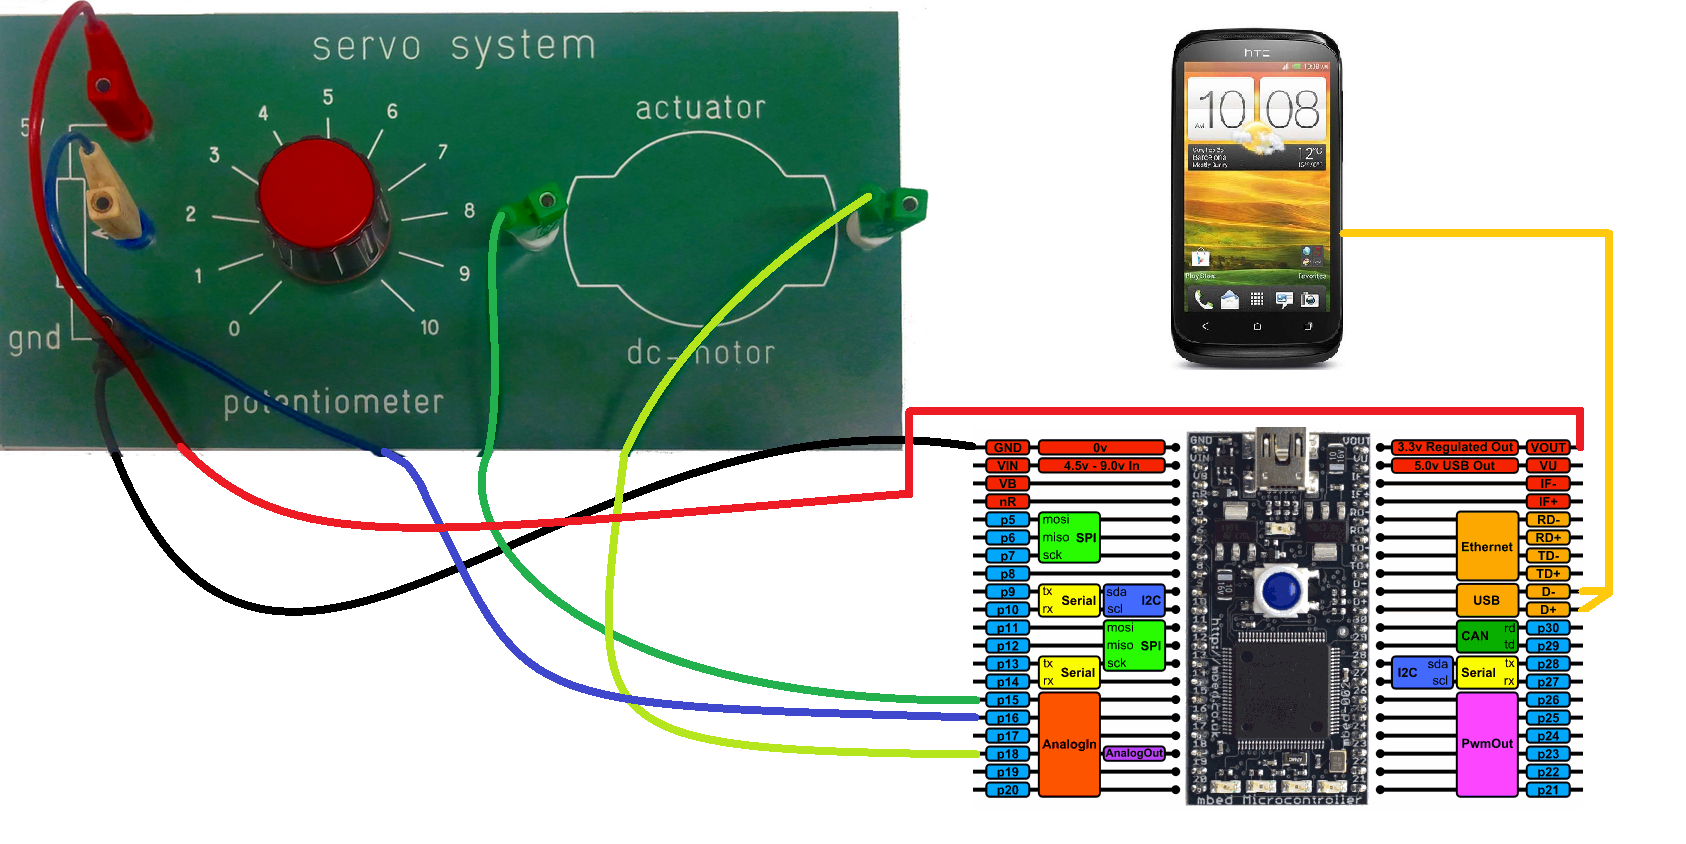
\includegraphics[width=0.8\textwidth]{imgs/opstelling.png}
		\caption{Opstelling}
		\label{fig:opstelling}
	\end{figure}
	\section{Onderzoek}
		Het is noodzakelijk eerst te onderzoeken hoe het servo systeem werkt. De analoog zichtbare waardes op het servo systeem lopen van nul tot tien. De potentiometer geeft echter een waarde tussen nul en \'e\'en af aan de mbed. om het verband tussen de analoge waarde en de mbed te bepalen moeten er metingen worden gedaan. De knop op het servo systeem kan op een bepaalde stand worden geplaatst. Vervolgens kan de waarde van de potentiometer getoond worden. Er worden elf metingen gedaan vanaf de waarde nul tot en met tien. De waarden zijn terug te vinden in tabel \ref{tab:gemeten}, de bijbehorende grafiek staat in figuur \ref{fig:logaritmisch}. Uit de gemeten waarden valt af te lezen dat het servo systeem exponentieel in waarde stijgt in plaats van lineair. Aan de hand van een vergelijking zou de waarde geschat kunnen gaan worden die de servo moet gaan aannemen bij de bijbehorende analoge stand. Het blijkt echter beter te werken om lineair te interpoleren tussen bekende waardes.
	\begin{table}[h]
		\begin{centering}
			\begin{tabular}{| c | c |}
				\hline
				Analoge waarde & Potentiometer waarde \\ \hline\hline
				1 & 0.002 \\\hline
				2 & 0.0062 \\\hline
				3 & 0.018 \\\hline
				4 & 0.059 \\\hline
				5 & 0.105 \\\hline
				6 & 0.2 \\\hline
				7 & 0.302 \\\hline
				8 & 0.504 \\\hline
				9 & 0.745 \\\hline
				10 & 0.996 \\
				\hline
			\end{tabular}
			\caption{Gemeten waarden}
			\label{tab:gemeten}
		\end{centering}
	\end{table}
	\begin{figure}[h]
		\centering
		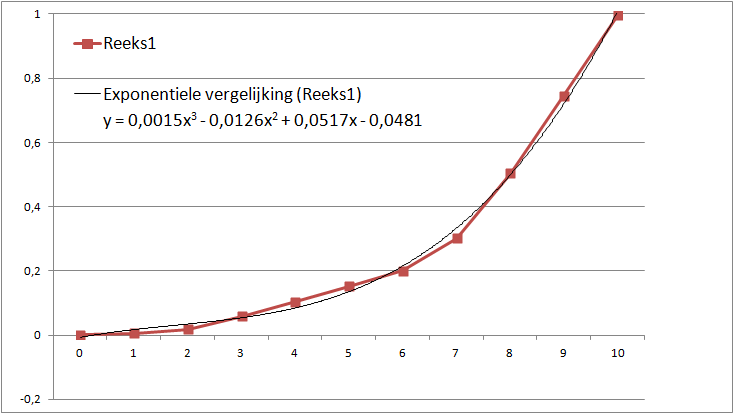
\includegraphics[scale=0.8]{imgs/logaritmisch.png}
		\caption{Exponentiele vergelijking}
		\label{fig:logaritmisch}
	\end{figure}
	\section{Logboek}
		\subsection{Maandag 3 Juni}
			Begonnen met het vertrouwt raken met de mbed. Enkele oefenprogramma's gemaakt die aangestuurd konden worden door middel van knopjes op de mbed zelf. Nog geen mogelijkheid gehad om waardes van de mbed naar de computer te krijgen. De lab machines die gebruikt konden worden hadden hiervoor geen permissies en er was geen eigen laptop meegenomen. Als tijdige oplossing output gecreerd door signalen met de LED lampjes.
		\subsection{Dinsdag 4 Juni}
			Programma's aan de praat gekregen die communiceren met een laptop. Juiste voltage en analoge waarde grafiek opgesteld. Android omgeving geinstalleerd. De voorbeeldcode voor een Android applicatie gecombineerd met mbed code onderzocht. Vervolgens begonnen met de layout van de Android applicatie en de mogelijkheden die er in de Android applicatie moeten komen.
		\subsection{Woensdag 5 Juni}
			Applicatie voor de Android werkend gekregen. De applicatie kan nu waardes aan de mbed doorgeven. De mbed zoekt vervolgens met deze waarde de juiste positie voor de as van de elektromotor. Begonnen met een server client systeem. De android die aangesloten staat op de mbed functioneert als server. Andere android toestellen met dezelfde applicatie zouden contact moeten kunnen leggen met deze android om de waardes van servo aan te kunen passen. Dit werkt echter nog niet.
		\subsection{Donderdag 6 Juni}
			Bijwerken en opschonen van het LabReport. Debugging lines toegevoegd aan de client server code voor de applicatie.
		\subsection{Vrijdag 7 Juni}
	
\end{document}